\section{Tömítés kiválasztása}

\subsection{Minimális tömítőerő}

\begin{align}
	&z = \frac{{d_2}_t - {d_1}_t}{2} = \siunit{\tomz}{db} \\
	&b_t^* = 9 + 0.2z = \siunit{\tombtstar}{\mm}
\end{align}

\begin{align}
	&F_\text{cső} 
	= \frac{\text{DN}^2 \pi}{4} p_\text{ü} = \n{\tomcso} \\
	&F_\text{p} 
	= \frac{\left(d_t^2 - \text{DN}^2\right)\pi}{4} p_\text{ü} 
	= \n{\tomp} \\
	&F_\text{töm} = n_t p_\text{ü} \pi d_t b_t^* = \n{\tomtu}
\end{align}

\begin{equation}
	F_\text{csavar üzemi} 
	= F_\text{cső} + F_\text{p} + F_\text{töm} 
	= \n{\csavaruzemi}
\end{equation}

\begin{align}
	&n_\text{bizt} = \siunit{\csavarn}{-} \\
	&F_\text{csavar szerelési} 
	= n_\text{bizt} F_\text{csavar üzemi}
	= \n{\csavarszerel}
\end{align}

\newpage
\subsection{Szabvány -és anyagválasztás}
% TODO

\newpage
\subsection{Előterv}
\begin{figure}[hbt!]
	\centering
	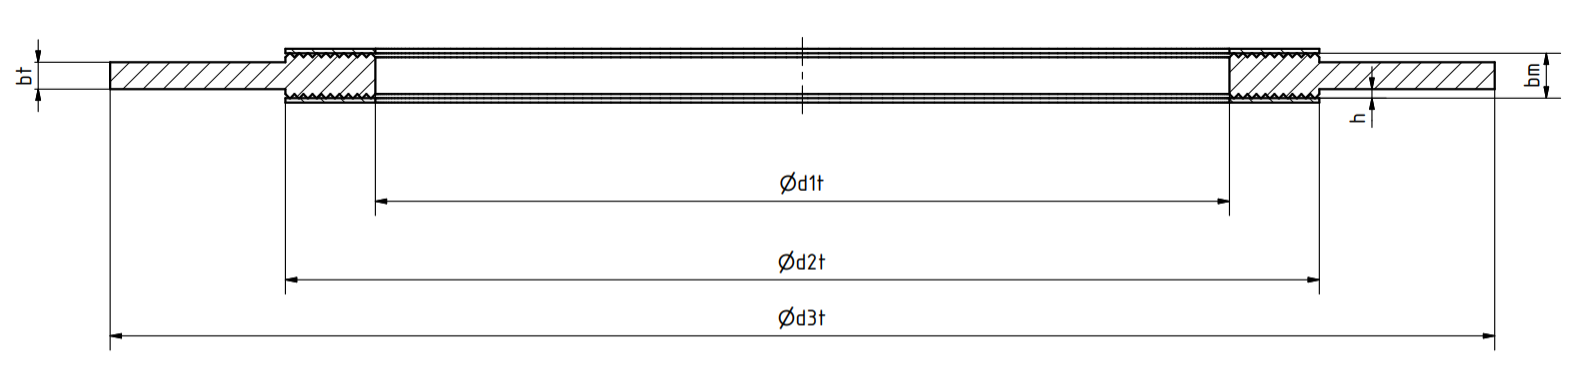
\includegraphics[scale=.34]{./images/tomites.png}
	\caption{Tömítés előtervének rajza}
\end{figure}
\begin{align*}
	&d_1 = \siunit{\tomdone}{\mm} \\
	&d_2 = \siunit{\tomdtwo}{\mm} \\
	&d_3 = \siunit{\tomdthree}{\mm} \\
	&b_t = \siunit{\tombt}{\mm} \\
	&b_m = \siunit{\tombm}{\mm} \\
	&h_{\text{max}} = \siunit{\tomhmax}{\mm} \\
	&h_{\text{min}} = \siunit{\tomhmin}{\mm}
\end{align*}
